\chapter{Method}\label{method}
We evaluated our models on the task of predict the sentiment of movie reviews.
We used SST with binary setting (See Sec.\ref{sec:sst}) to train and evaluate our models. 

\begin{table}[H]
	\centering
	\caption{Number of trainable parameters of experimented models}
	\label{table:paramtable}
	\begin{tabular}{lll}
		~ & Memory Size of RNNs unit & Parameters count \\ \hline
		LSTM                     & 168         & 315,840          \\
		BiLSTM                   & 168         & 315,840          \\
		Constituency Tree-LSTM   & 150         & 316,800          \\
		Dependency Tree-LSTM     & 168         & 315.840          \\
		Constituency VT Tree-GRU & 150         & 476,103          \\
		Dependency VT Tree-GRU   & 150         & 316,353          \\
		CNN LSTM                 & 168         & 489,347          \\
		CNN Tree-LSTM            & 150         & 482,153          \\
		2 channel CNN LSTM       & 168         & 729,347          \\
		2 channel CNN Tree-LSTM  & 150         & 722,153         
	\end{tabular}
\end{table}

\section{Models Description}
\subsection{Model VT Tree-GRU}\label{sec:VTtree}
\begin{figure}[H]
	\centering
	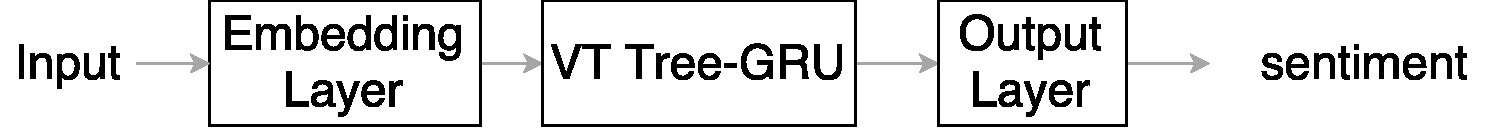
\includegraphics[width=0.8\linewidth]{figure/vtgrusummary.pdf}
	\caption[Convolution Tree LSTM]{}
	\label{fig:vtgrusummary}
\end{figure}

\subsubsection{Embedding layer}\label{sec:embedding}
Embedding layer is a lookup table that convert input data (such as text) into its vector representation. A word embedding layer parameters is its embedding matrix $M  \in \mathbb{R}^{n \times d}$, where $n$ and $d$ is vocabulary size and embedding vector dimension, respectively. In practical, an embedding layer also come with vocabulary-index lookup table, which map word with index, which has vector representation corresponding to row in word embedding matrix.
  
The following step are require once for each experiment:
\begin{itemize}
	\item Build vocabulary-index lookup table
	\item Init/Load word embedding matrix corresponding to vocabulary-index table
	\item Convert every sentences in dataset into indices using vocabulary-index table  
\end{itemize}
Usually, indices are keep as dataset. Raw dataset (such as readable words) are discarded to free up memory. For each mini-batch, we use indices to lookup word representation vector from embedding matrix. Embedding matrix represent of each sentences in dataset are not saved and needed look-up every mini-batch for following reason.
\begin{itemize}
	\item Saved embedding matrix for each data sentences cost more memory than save only indices and look-up in embedding layer.
	\item Embedding matrix are trainable parameters and updated every iteration.
\end{itemize}

Fig.\ref{fig:embeddinglayer} illustrates embedding layer component and describes the process of convert raw data sentence into its word representation.

\begin{figure}[H]
	\centering
	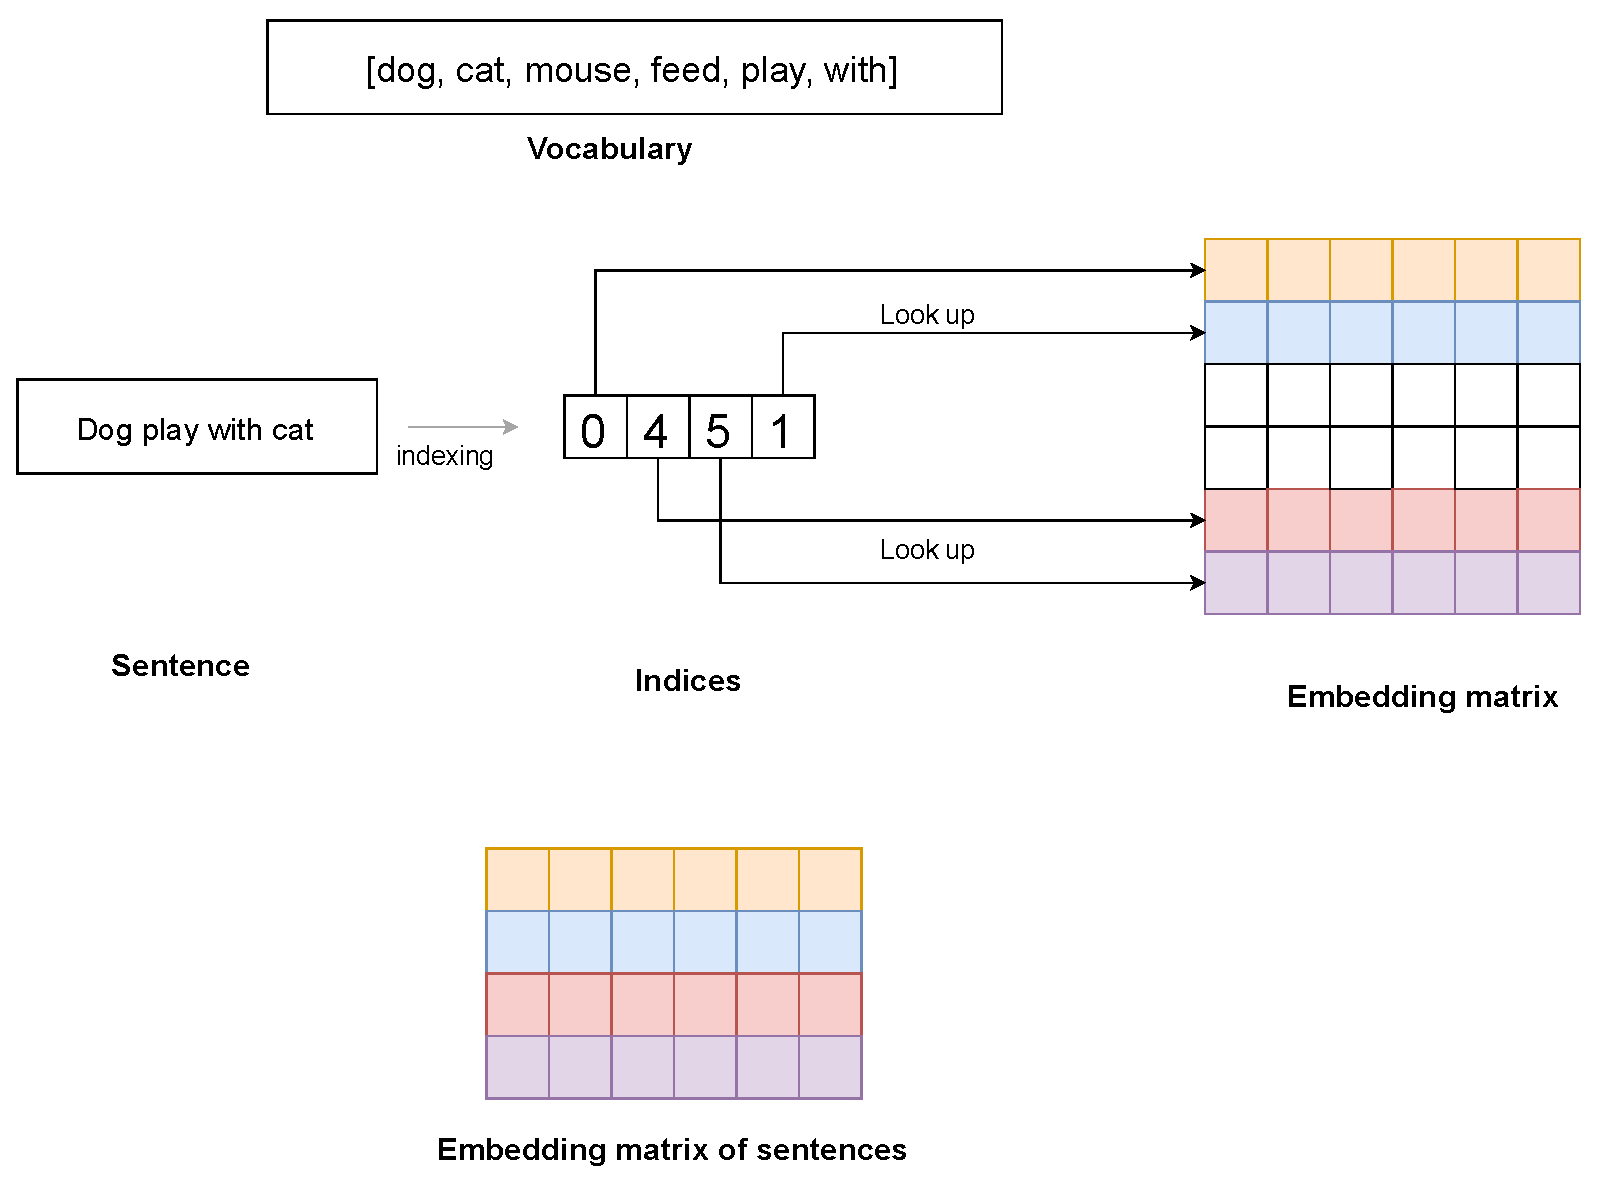
\includegraphics[width=0.9\linewidth]{figure/embeddinglayer.pdf}
	\caption[Overview of embedding layer]{Overview of Embedding Layer}
	\label{fig:embeddinglayer}
\end{figure}



\subsubsection{VT Tree-GRU}
We apply both tree structure network and recurrent structure in our model. In each sub-tree, which consist of one parent node with or without children, we apply recurrent network structure over current node and all its child. We store last hidden layer as node intermediate information and use as input to higher level. For network unit, we choose Gated Recurrent Unit (GRU), which was first introduced in \cite{cho2014learning}. GRU transition equation are describe in Eq.\ref{eq:gru}. 

\begin{equation}
\label{eq:gru}
\begin{aligned}
&r = sigmoid(W_{ir} x + b_{ir} + W_{hr} h + b_{hr}) \\
&i = sigmoid(W_{ii} x + b_{ii} + W_{hi} h + b_{hi}) \\
&n = \tanh(W_{in} x + b_{in} + r * (W_{hn} h + b_{hn})) \\
&h' = (1 - i) * n + i * h\\
\end{aligned}
\end{equation}

\subsubsection{Constituency VT Tree-GRU} \label{sec:VTtreeConstituency}
SST (See Sec.\ref{sec:sst}) given format is binary constituency parse tree. We use CoreNLP \cite{manning2014stanford} to create non-binary constituency parse tree and annoted Part-of-speech tag (POS-tag) for each node. We use word and tag and tree structure as input for our model.

For each sub-tree, we sort child node from left to right order. We take node state k, node POS-tag, and parent POS-tag as input for GRU timestep. We put parent node at the end of GRU chain. We take hidden state of last timestep as node state k for parent node. For a sub tree Fig.\ref{fig:treecp}, model is illustrate in Fig.\ref{fig:cvtgru}. For leaf node case, we input word and tag into GRU and get hidden output h as k for leaf node as Fig.\ref{fig:gruleaf}.
\begin{figure}[H]
	\centering
	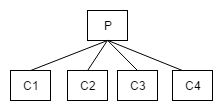
\includegraphics[width=0.5\linewidth]{figure/treecp}
	\caption[A sub tree with parent and children node]{A sub tree with parent and children node}
	\label{fig:treecp}
\end{figure}

\begin{figure}[H]
	\centering
	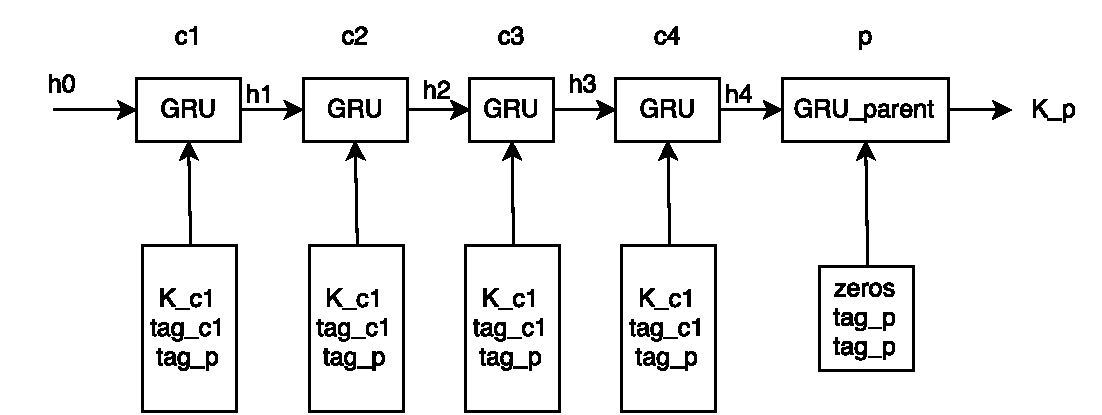
\includegraphics[width=0.9\linewidth]{figure/cvtgru}
	\caption[Constituency VT Tree-GRU]{Constituency VT Tree-GRU}
	\label{fig:cvtgru}
\end{figure}

\begin{figure}[H]
	\centering
	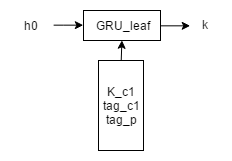
\includegraphics[width=0.4\linewidth]{figure/gruleaf}
	\caption[Constituency VT Tree-GRU leaf case]{Constituency VT Tree-GRU leaf case}
	\label{fig:gruleaf}
\end{figure}



\subsubsection{Dependency VT Tree-GRU} \label{sec:VTtreeDependency}
We use \cite{manning2014stanford} to create dependency parse tree with annoted POS-tag and labeled Universal Dependencies between head word and its dependents.

We build a model similar to constituency case, with a chain GRU for each sub tree. However, we does not put parent node at the end of the chain. Instead, parent node and child node are sorted according to their position in sentences. We take node state k, node POS-tag, node dependency relationship type vs head word as input for GRU timestep. At parent node, we set dependency relationship type is 'self' and node states k set to zeros vector. We take hidden state of last timestep as node state k for parent node. In case of leaf node, we treat it as parent node without children. We build GRU chain with only parent node for leaf case. Fig.\ref{fig:dependencyvtgru} illustrate Dependency VT GRU model.

\begin{figure}[H]
	\centering
	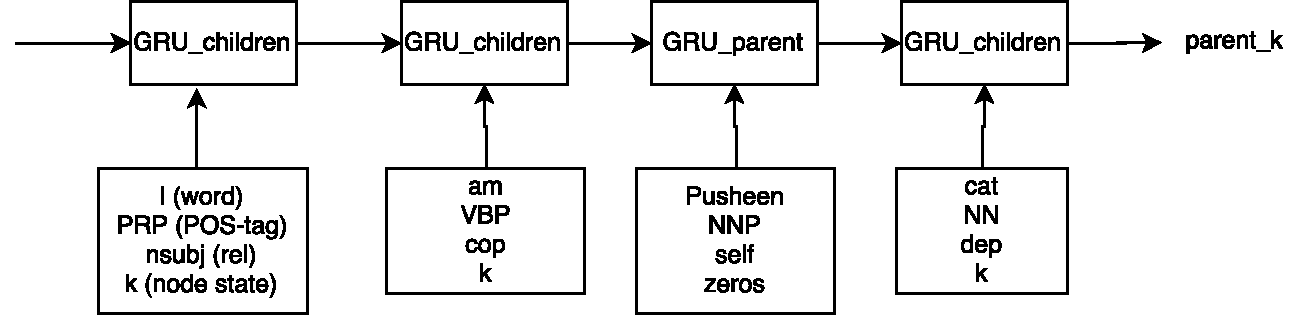
\includegraphics[width=0.9\linewidth]{figure/dependencyvtgru}
	\caption[Dependency VT Tree-GRU]{Dependency VT Tree-GRU}
	\label{fig:dependencyvtgru}
\end{figure}

\subsubsection{Output layer and loss function}
We use softmax classifier and cross entropy loss function as described in \cite{treeLSTM}.  For each parent labeled node, we use node state $k$ as input to output layer and calculate loss against given label. Root node state $k$ is used to determine sentiment of whole sentences.


\subsection{CNN-TreeLSTM and CNN LSTM}\label{sec:CNNtree}

\begin{figure}[H]
	\centering
	
\includegraphics[width=0.8\linewidth]{figure/convtreelstmsummary}
	\caption[Convolution Tree-LSTM overview]{Convolution Tree-LSTM overview}
	\label{fig:convtreelstmsummary}
\end{figure}
Based on our discussion on \hyperref[sec:tree-discuss]{tree-structured vs. sequential} network architects and \hyperref[kim-cnn]{the benefits of using Convolution layer}, we combined \hyperref[conv-filter]{Convolution layer} with \hyperref[sec:treelstm]{Tree-LSTM}\cite{treeLSTM}.
We hypothesized that, the convolution layer will help Tree-LSTM to mitigate the problem of lacking local context and weak feature capturing at leaf nodes.
Additionally, using Tree-LSTM to combine the feature maps produced by Convolution layer is better than \hyperref[sec:max-overtime-pooling]{max-over-time pooling layer}.
The increased model complexity can lead to over-fitting, to tackle this risk, we can unsupervised pre-train the models using methods described in Sec.\ref{sec:unsupervised-pretrain}.

We keep embedding layer, output layer and Tree-LSTM as same as TreeLSTM implementation.
We also replace Tree-LSTM with \hyperref[sec:lstm]{LSTM} to make CNN-LSTM model, which is similar to \hyperref[cnn-rnn]{Wang's models}\cite{cnn-rnn}.  
The reason we want to do experiment with CNN-LSTM model is because CNN-LSTM can be unsupervised pre-trained as Language Model, while Tree-LSTM can not (Sec.\ref{sec:unsupervised-pretrain}).

\subsubsection{Convolution layer implementation} \label{sec:conv1c}
Each convolution layer contain n filter. Each filter has dimension $wd$, with \(d\) is word vector dimensions and \(w\) is word-level kernel size. 
We may have one or more kernel size, with are treat as models' hyper-parameter. 

We aligned the first axis of each feature map with the embedding axis and convolved along first dimension of embedding matrix. 
We useed 'half' convolutions~\footnote{'half' padding policy: http://deeplearning.net/software/theano/tutorial/conv\_arithmetic.html} with unit strides, which each filter produce a 1d vector have same length as sentence length. 
Thus, n filter produces $l x n$ matrix with $l$ is sentence length. We set $n = d$ in order to produce output with same dimension as embedding matrix. We use ReLU activation function \cite{hahnloser2000digital}. Fig \ref{fig:convlayer} illustrates convolution process. 



\begin{figure}[H]
	\centering
	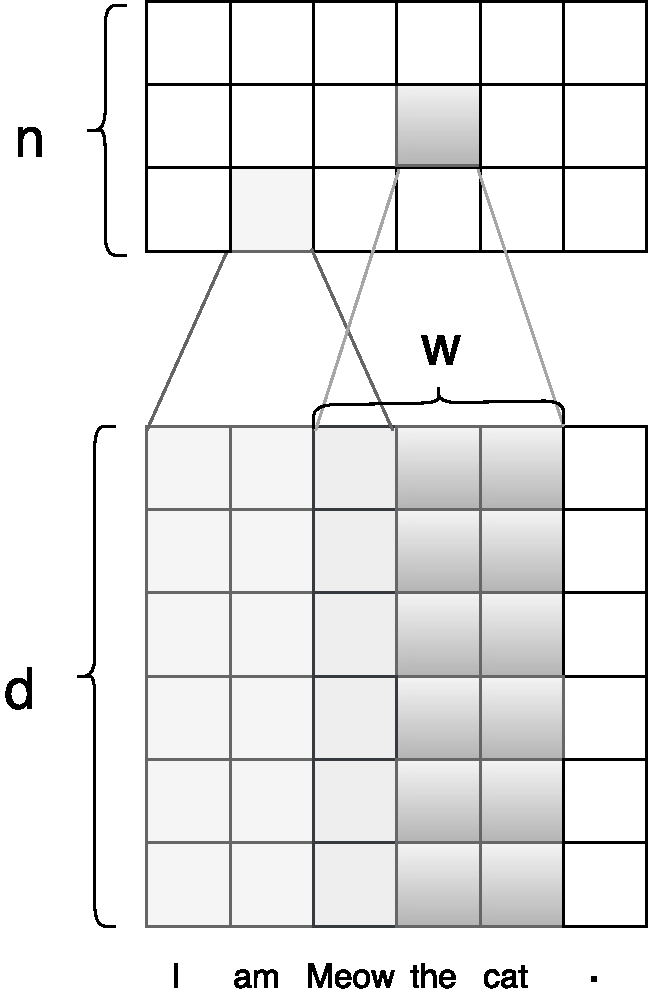
\includegraphics[width=0.4\linewidth]{figure/convlayer}
	\caption[Convolution layer]{Convolution layer}
	\label{fig:convlayer}
\end{figure}

\section{Models Enhancements}
\subsection{Training Glove embedding on Amazon reviews dataset}\label{sec:gloveamazone}
There are many words (e.g. "B-rated", "Lolita", "Nolan", "cartoonlike") which rarely appears in regular documents but more often in movie reviews.
We hypothesize that using review documents, especially movie or book reviews, we can capture more rare words and also the different way people use words (or different word relationships) when they express their opinions on movies or books.
We chose \hyperref[sec:glove]{Glove method} for archiving this purpose.
\paragraph{Steps for preprocessing Amazon dataset for training Glove vectors}
\label{sec:preprocessamazonglove}
\begin{enumerate}
\item For retraining Glove vectors, we only used Amazon Movies and TV reviews dataset (7,850,072 reviews)\cite{mcauley2013hidden}, Amazon Book reviews(22,507,155 reviews) and new Movies and TV dataset (4,607,047 reviews)\cite{McAuleyTSH15}\cite{HeM16}.
\item All the reviews were grouped by product-ID ("asin" keyword in the \hyperref[sec:amazon]{JSON schema of the dataset}). 
\item In each product-ID group, the reviews were sorted increasingly by their rating ("overall" keyword in the JSON schema of the dataset).
\item All the reviews were dumped into a plain text file.
\item The text file produced from the previous step was tokenized using Stanford Tokenizer \cite{tokenizerpart}. 
\end{enumerate}

\paragraph{Training method and hyper-parameters}
We use Glove implementation \footnote{Publicly available on Github \url{https://github.com/stanfordnlp/GloVe}} to train word representation. 
We set $x_{max} = 100$, vector size to 300, windows size to 20 and minimum number of word occurrences to be included in the vocabulary to  5.
The training process took the plain text file produced by the \hyperref[sec:preprocessamazonglove]{preprocessing steps} as its input. 
In total, the size of the corpus is 4.7 billions tokens. 
After the training process, the resulting word embeddings has vocabulary size of 1,734,244.

\subsection{Using multi-channel word embeddings}\label{sec:enhan-multi-channel}
This method was introduced by Yoon Kim\cite{KimCNN}.
The description and analysis of this method can be found in Sec.\ref{kim-cnn}.
The type of word embeddings used in each channel, the number of channels and the method for updating each channel are treated as hyper-parameters.

This method allowing multiple parallel embedding layer in our model. 
In other words, each word have two vector representation. 
The method allows two pre-trained word representation. 

\begin{figure}[H]
	\centering
	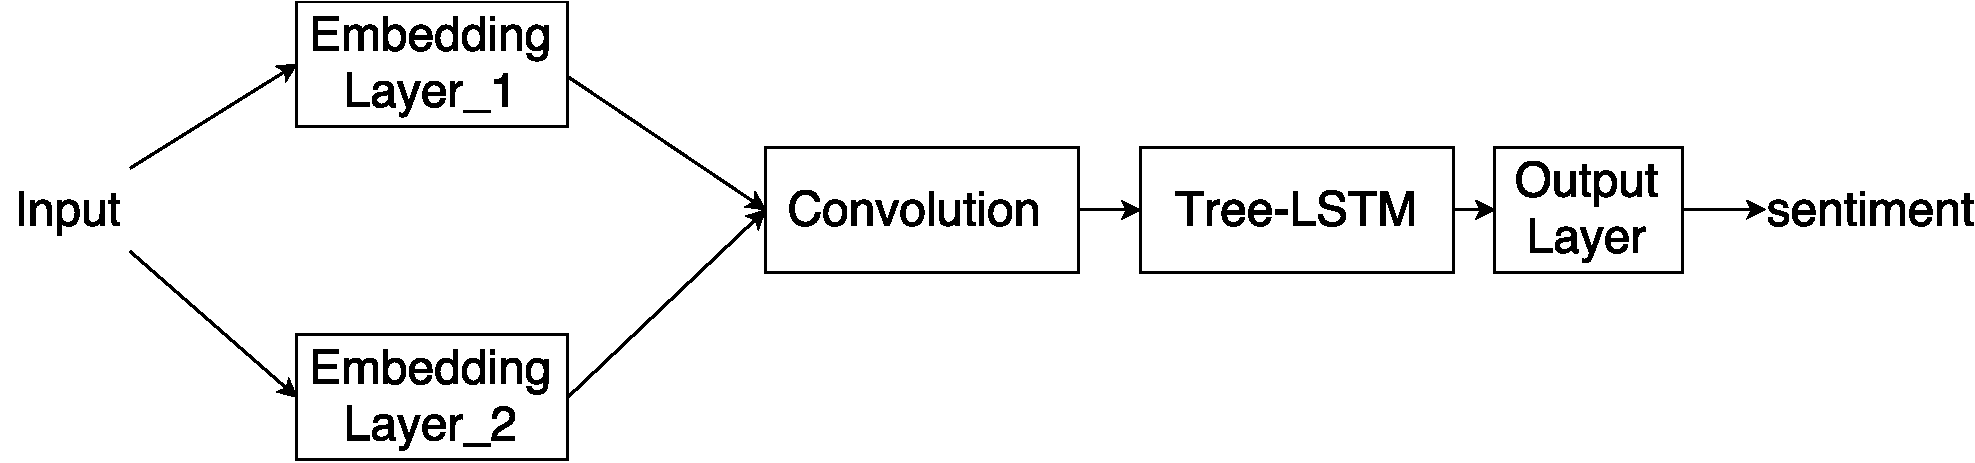
\includegraphics[width=0.8\linewidth]{figure/multichannelcnnlstm}
	\caption[Convolution Tree-LSTM overview]{Two input channel Convolution Tree-LSTM overview}
	\label{fig:multichannelcnnlstm}
\end{figure}


\subsection{Pre-training models as Language Models on Amazon reviews dataset}
In Sec.\ref{sec:unsupervised-pretrain}, we have already presented several methods for unsupervised pre-training neural network models and given some hypotheses on the beneficial effects of these methods.
\paragraph{Steps for preprocessing Amazon dataset for training Language Model}
\label{sec:preprocessamazonglove-LM}
\begin{enumerate}
\item For retraining Glove vectors, we only used new Movies and TV dataset (4,607,047 reviews)\cite{McAuleyTSH15}\cite{HeM16}.
\item All the reviews were grouped by product-ID ("asin" keyword in the \hyperref[sec:amazon]{JSON schema of the dataset}). 
\item In each product-ID group, the reviews were sorted increasingly by their rating ("overall" keyword in the JSON schema of the dataset).
\item A special character sequence was added at the end of each review to mark its end.
After that, all the reviews were dumped into a plain text file.
\item The text file produced from the previous step was tokenized using Stanford Tokenizer \cite{tokenizerpart}. 
\item The tokenized text file was then divided into training and test set using 95:5 split.
Because this is an pre-training process, we used only 5\% of the data to test if the Language Model was trained properly.
\end{enumerate}


\section{Our Experiments}
\subsection{Evaluate VT-Tree SST datasets}
\subsubsection{Training method and hyper-parameter}
We preprocess SST as described in Sec.\ref{sec:VTtreeConstituency} and Sec.\ref{sec:VTtreeDependency}. We use default train/dev/test split after remove neutral sentences (6920/872/1821). We only remove neutral sentence, but keep neutral text span of positive or negative sentences. We fine tune our model on development dataset using gird search.

We initialized our word representation with pretrained word vector (Glove \footnote{Common Crawl (840B tokens, 2.2M vocab, cased, 300d vectors, 2.03 GB download) publicly available at \url{https://nlp.stanford.edu/projects/glove/}} \cite{glove}, paragram\_xxl \footnote{50,000 embeddings, publicly available at \url{http://ttic.uchicago.edu/~wieting/}} \cite{wieting2015towards}) with default dimension of 300.  We initialize randomly tag and relationship representation (dependency only) vector of dimension 50. We set memory dimensions of 150. 

Our model was trained using AdaGrad \cite{duchi2011adaptive} with learning rate of $\{0.1,~ 0.05,~ 0.01\}$ and Adam $\{1e^{-3}, 1e^{-4}\}$, L2 regularization strength of $\{1e^{-3},~ 1e^{-4}, ~ 1e^{-5} \}$, batch size of 25. We manually update our word representation with learning rate $\alpha$ of $\{0.1,~0.05, ~0.01\}$ as Eq.\ref{eq:manuallyupdate}. In addition, we used dropout \cite{krizhevsky2012imagenet} to regularize our model. We regularized Tree-GRU with input dropout rate of 0.5 and memory dropout rate at 0.1. Sentiment classifier was also regularized with 0.5 dropout rate. 
\subsection{Evaluate CNN Tree-LSTM SST datasets}
\subsubsection{Training method and hyper-parameter}
We initialized word representation with Glove vectors\cite{glove}. 
With two word embeddings channels, we initialized one channel using Glove Common Crawl\footnote{\label{glovecommoncrawl}Common Crawl (840B tokens, 2.2M vocab, cased, 300d vectors, 2.03 GB download) publicly available at \url{https://nlp.stanford.edu/projects/glove/}} and the other using our Glove vectors trained on Amazon dataset (Sec.\ref{sec:gloveamazone}). 

We tried a variety of convolution filters combination. For single kernel size, we performed gird search on $\{100, 200, 300\}$ kernel of size $\{3, 5\}$. For two different kernel size, we tried with $\{100, 200\}$ number of filter for each filter kernel size. Output matrix of different kernel size was concatenated as it was with same kernel size. 

Our model was trained using AdaGrad \cite{duchi2011adaptive} with learning rate of $\{0.1,~ 0.05,~ 0.01\}$, L2 regularization of $\{1e^{-3},~ 1e^{-4}, ~ 1e^{-5} \}$, batch size of 25. We manually update our word representation with learning rate $\alpha$ of $\{0.1,~0.05, ~0.01\}$ as Eq.\ref{eq:manuallyupdate}. We regularized convolution layer with input dropout rate of 0.5 and output dropout rate of 0.2 in addition to dropout of rate 0.5 at dropout layer. 
We apply same gird search parameters for two channel convolution. 
\begin{equation}
\label{eq:manuallyupdate}
w = w - \alpha\delta J(\theta)
\end{equation}